\documentclass{article}
\usepackage{graphicx, subfigure, multirow}
\usepackage{amsmath,cite}
\usepackage{amsthm}
\usepackage{tikz}
\usetikzlibrary{arrows}

%\renewcommand{\arraystretch}{1.5}
\newtheorem{mydef}{Definition}

\title{Solving small shogi}%TODO fix title
\author{Ingo van Duijn \\ Utrecht University}
\begin{document}
\maketitle

\begin{abstract}
Shogi is a popular chess variant in Japan. Though similar to chess, in shogi the drop rule allows captured pieces to be dropped on the board by the captor. As such,
not all techniques from computer chess work equally well on shogi. Techniques have to be adapted or new ones tailored
to be suited for shogi. In this paper we will investigate the viability of using proof-number search to find the game theoretical value of
small variants of shogi. Both an unadapted and an adapted version of this method will be described. Both version outperformed a basic implementation
of the minimax algorithm on $3 \times 3$ boards, though the adapted version solves less instances. On a larger $3 \times 4$ variant, both versions
do not look promising. The unadapted version could not handle the combinatorial explosion the drop rule introduced. The adapted version solves this
by representing the game tree as a graph, however proof-number search does not work well on graphs. 
%TODO finishing sentence
\end{abstract}

\section{Introduction}
Ever since the early days of modern computers there has been great interest in chess programming. Initial
focus in the west was mainly on chess and checkers, but when computers were well established in Japan, researchers there adopted
many techniques from computer chess and applied them to their local chess variant, shogi.

\subsection{Shogi}
Shogi (Japanese chess\cite{shogibook}) is a game similar to western chess. It is played on a $9 \times 9$ board and every
player has 20 pieces, some of which correspond to western pieces and others are slightly different.
Black makes the opening move and both players aim to capture the opponent's king.
The main difference between shogi and chess is the so called \emph{drop rule}.
A piece that is captured by a player now belongs to him and can be placed on \textit{any} vacant square in one of his subsequent turns
(in stead of moving a piece already on the board).
Additionally, in shogi nearly all pieces can promote upon moving to or from the promotion zone (starting ranks of opponent).
Unlike western chess, each type of shogi piece can only be promoted to one specific type of piece (e.g. a bishop always promotes to a dragon horse).
The drop rule, and to a lesser extent the promotion rule, dramatically increase the game tree complexity of shogi as compared to chess, see Table
\ref{table:complex} for a comparison.\\
\begin{table}
\center
\begin{tabular}{l l l l}
 & Chess & Shogi & Go \\ \hline
State-space complexity & $10^{43}$ & $10^{71}$ & $10^{172}$ \\
Game-tree complexity & $10^{123}$ & $10^{226}$ & $10^{360}$ \\ \hline
\end{tabular}
\caption{The complexities of chess, shogi and go}
\label{table:complex}
\end{table}

\subsection{Computer shogi}
Like computer chess, computer shogi is an active field of research~\cite{iida2002computer}. The main interest is how we can program computers 
such that their play peers with -- and eventually even surpasses -- human professional players. Shogi, being complexer
than western chess, has a game tree much too large for exhaustive search. Consequently, research
focusses on clever ways to search the game tree in order to find a good heuristic. Many techniques from computer chess
have been employed, but the drop rule introduced such a novelty that new shogi-specific techniques had to be developed.\\

Unlike in western chess, end game situations
in shogi are not significantly less complex than mid game situations. In fact, any board configuration resulting from the standard
starting setup has exactly 40 pieces in play. Because of this there is no database with solved end games for shogi.
However, in shogi, so called mating problems \footnote{On a predesigned setup, black (lacking a king) can only make checking moves},
which resemble end game situations, are extensively studied ~\cite{grimbergen1999survey}. There exist several
programs that can completely solve a lot of these problems, some of which are quite large\footnote{The largest mating problem needs 1525 plies to solve}
~\cite{seo2001pn}. Unfortunately solutions to these shogi
mating problems are not the equivalent of solutions to western chess end games; in shogi, such a solution cannot be directly applied to find a winning move.
However, since the methods used to prove the shortest mating sequence are exact and not heuristical, they or similar methods might be useful to prove
certain subsets or small variants of shogi.\\

\subsection{Solving small shogi variants}
Even though end game situations in shogi are quite complex, there are of course enough situations advanced enough -- near victory -- that they
should be perfectly solvable. For instance if no move of the losing player can check the opposing king, it might be possible to restrict the search
for the optimal move to a subset of the board. We are going to emulate this by actually looking at shogi variants played on a smaller board
altogether.

One particular method, proof-number search, has been proved to be quite effective, even outperforming $\alpha\beta$-search~\cite{van2008proof} in
proving the game theoretical value of a game tree. This method has also been succesfully applied to shogi mating
problems~\cite{seo2001pn, ueda2008weak, sakuta2001performance}. We will discuss the viability of using proof-number search to solve variants of shogi and will test
this method on small shogi variants.

\subsection{Contents}
Section \ref{sec:rep} will contain a description of a generic way to describe small shogi variants. In Section \ref{pnsearch} we will introduce proof-number
search, followed by a more formal definition accompanied by pseudo-code. It concludes with a description of each implemented method.
In Section \ref{sec:results} we will describe the test domains and present the performance of each method with relevant figures.
An interpretation of these results will be discussed in Section \ref{sec:disc}. We will conclude with suggestions to further improve
proof-number search for use with shogi.%TODO verify this last sentence

\section{Method}
We are dealing with generic small sized shogi variants, so representation and algorithms employed have to be sufficiently generic as well.
A small shogi variant is defined by the size of the board, the initial configuration of black, for white's is $180^{\circ}$ rotationally symmetrical, and
the size of the promotion zone. The initial configuration consists of a set of pieces, each of which has one or two move sets; a normal move set and
its promoted move set. An algorithm that aims to prove the game theoretical value of such a shogi variant only has to have access to two functions based on this
definition: a move generator which can map positions to a set of successing positions, and an evaluation function which recognises terminal
positions and computes their value.

\subsection{Representation}
\label{sec:rep}
As stated before, we have to be able to generically represent board positions. A well known technique in computer chess, bitboards, has been
shown~\cite{grimbergen2007using} to be fairly effective in shogi as well. A bitboard is a bit pattern of at least the size of the board,
in which each bit encodes some information about the corresponding square, e.g. if it is occupied.
Figure \ref{bitsquares} shows the correspondence between squares and bits, zero being the least significant bit.
Since the size of the bit pattern can
easily be increased to accomodate larger boards, they are well suited for our purpose. Also, as will be explained later, they allow for easy
generic move generation.

\begin{figure}
\center
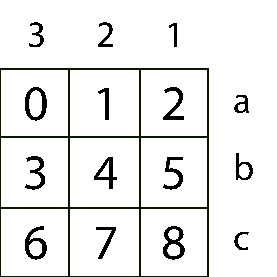
\includegraphics{bitsquares.pdf}
\caption{Correspondence between squares and bits on a $3 \times 3$ board.}
\label{bitsquares}
\end{figure}

In the current implementation, a position is represented by the following: per player one bitboard for every piece's normal and possibly promoted move set, 
additional to one bitboard for both players containing the pieces in hand, viz. pieces that can be dropped by that player.
Each bitboard corresponding to a certain piece's move set represents all pieces of that type
owned by a specific player. Figure \ref{bitboard} shows an example configuration on a $3 \times 3$ board with the
bitboard representing black's pawns. For an $n \times m$ board, each bitboard is fitted in the smallest $nm \leq 2^k$-bit integer, so for small
variants $16$ or $32$ bit integers suffice.

\begin{figure}[h]
\center

    \mbox{
      \subfigure[Example starting configuration]{\label{3x3setup}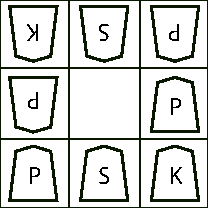
\includegraphics{smallsetup.pdf}} \quad
      \subfigure[Bitboard of black's pawns]{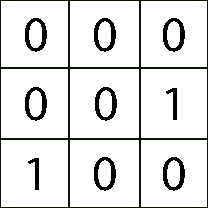
\includegraphics{blackpawnbits.pdf}}
      }

\caption{An example of how a bitboard captures some information of the board position.}
\label{bitboard}
\end{figure}

To generate moves, we essentially need two things. We need to know for each individual piece where it is, and where it can move to in its current state.
The location of each individual piece can be extracted from the bitboard corresponding to that piece's type. To determine where it can move to, a table
is generated which maps position bitboards to move bitboards. In Figure \ref{moveboard} is an example of all the possible moves of one of black's silver
generals positioned on b3. These tables are generated beforehand and are the basis of the move generator.

\begin{figure}[h]
\center
    \mbox{
      \subfigure[A silver general owned by black]{\label{blacksilver}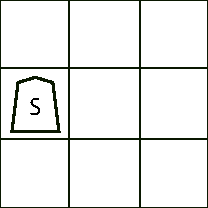
\includegraphics{blacksilver.pdf}} \quad
      \subfigure[All possible moves of the silver general]{\label{blacksilvermove}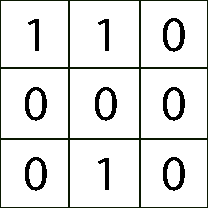
\includegraphics{blacksilvermove.pdf}}
      }
\caption{A silver general positioned on b3 can move to a3, a2 and c2.}
\label{moveboard}
\end{figure}

Finally, the evaluation function can use the move generator to check whether any move captures the opponent's king. Note that the evaluation function
does not give a heuristical value, it only evaluates terminal positions to nonzero values ($1$ for win and $-1$ for loss).

With the move generator and the evaluation function in place, we have an implicit definition of the game tree. The main problem of proving the game
theoretical value efficiently is only generating relevant parts of the tree.

\subsection{Proof-number Search}
\label{pnsearch}
Proof-number search~\cite{allis1994proof}, or PN-search, is an algorithm designed to find the game theoretical value of a game tree, or more specifically an AND/OR tree.
The tree consists of a root, internal nodes and leaf nodes. Each node is either an AND (white to move) or an OR node (black to move). By definition, a leaf
node represents one player's victory and thus it has a nonzero value of $1$ (black won) or $-1$ (white won). As in the minmax algorithm, an internal
node's value can be computed by taking the maximum or minimum of the children's value for AND and OR nodes respectively (Figure \ref{tree:simple}).

\begin{figure}[h]
\center
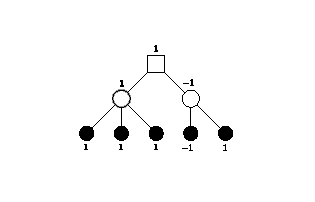
\includegraphics[width=10cm]{simpleminmax.pdf}
\caption{Square AND nodes, circular OR and filled terminal nodes with their respective value.}
\label{tree:simple}
\end{figure}
% \begin{figure}[h]
% \center
% \begin{tikzpicture}[
    % all/.style={minimum width=.5cm, minimum height=.5cm},
    % and/.style={all, circle, draw},
    % or/.style={all, rectangle, draw},
    % term/.style={circle, draw=black, fill},
% ]
    % \node [or, label=1] {} 
        % child { node [and, label=1] {} 
                % child { node [term, label=below:1] {} }
                % child { node [term, label=below:1] {} }
                % child { node [term, label=below:1] {} }
        % }
        % child {
            % node [and, label=-1] {}
            % child { node [term, label=below:-1] {} }
            % child { node [term, label=below:1] {} }
        % }
    % ;
% \end{tikzpicture}
% \caption{Square AND nodes, circular OR and filled terminal nodes with their respective value.}
% \label{tree:simple}
% \end{figure}

The most simple form of the minmax algorithm performs a depth-first expansion of the tree to calculate the value of the root. Proof-number search however
expands the tree in a \textit{best-first} manner untill the root can be proved (i.e. determining its game theoretical value). The algorithm starts with a single
unproved node, the root. It then successively picks the most promising unproved node and expands it, i.e. generating its children. Since terminal nodes are proved
directly upon generation, unproved nodes are never terminal and will have children once they are expanded. 

\subsubsection*{Most proving node}
The tree in Figure \ref{tree:pnex} has proved and unproved nodes. The nodes with a value are proved ($d$ and $g$) and the rest is unproved.
Since the root $a$ is an OR node, it suffices
to prove either $b$ or $c$. Both these nodes, being AND nodes, need the value of all their children before they can be proved. The sets of
unproved children for $b$ and $c$ respectively are $\{e, f\}$ and $\{h\}$. For the root, in stead of saying that we need to prove
either $b$ or $c$, we can also say we need to prove either $\{e, f\}$ or $\{h\}$. Since the latter set is smaller, it is more
promising trying to prove $c$ than it is to prove $b$. Repeating this argument for determining the most promising branch of the tree
eventually leads to an unproved node, $h$ in the example, which we call the \textit{most proving node}.\\

\begin{figure}[h]
\center
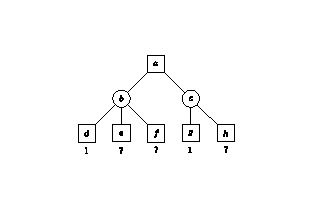
\includegraphics[width=10cm]{proofset.pdf}
\caption{Square AND nodes, circular OR, unproved nodes are labelled with a question mark.}
\label{tree:pnex}
\end{figure}
% \begin{figure}[h]
% \center
% \begin{tikzpicture}[
    % all/.style={minimum width=.5cm, minimum height=.5cm},
    % and/.style={all, circle, draw},
    % or/.style={all, rectangle, draw},
    % term/.style={circle, draw=black, fill},
% ]
    % \node [or] {$a$} 
        % child { node [and] {$b$} 
                % child { node [or, label=below:1] {$d$} }
                % child { node [or, label=below:?] {$e$} }
                % child { node [or, label=below:?] {$f$} }
        % }
        % child {
            % node [and] {c}
            % child { node [or, label=below:1] {$g$} }
            % child { node [or, label=below:?] {$h$} }
        % }
    % ;
% \end{tikzpicture}
% \caption{Square AND nodes, circular OR, unproved nodes are labelled with a question mark.}
% \label{tree:pnex}
% \end{figure}

Before we introduce the algorithm, a formal description of the most proving node is required.\\
The \textit{game tree} represents all possible ways to play the game. Whereas the \textit{search tree} is used by the algorithm
and only contains a portion of the game tree relevant for proving the root. The search tree grows as the algorithm expands nodes and
unproved expanded nodes are eventually either proved or disproved.
\begin{mydef}
If a node is proved it has game theoretical value $1$, indicating a win for the beginning player (Black).
Conversely, if a node is disproved it has value $-1$ and indicates a win for the opponent (White).
An unproved node can be an internal or leaf node of the search tree.
\end{mydef}

To define the most proving node we need a notion of how close a node is of being proved.
\begin{mydef}
Given a search tree, let $N$ be the set of its nodes and $L \subseteq N$ be the set of unexpanded nodes. A set $P \subseteq L$ is called a proof set of a node $v \in N$ if proving all $w \in P$ will prove $v$.\\
Similarly, a set $D$ is called a disproof set of a node $v$ if disproving all $w \in D$ will disprove $v$.\\
A proof set is called atomic if all its proper subsets are no longer proof sets.\\
Similarly, a disproof set is called atomic if all its proper subsets are no longer disproof sets.
\label{def:pset}
\end{mydef}
In the search tree in Figure \ref{tree:pnex}, the root has atomic proof sets $\{e, f\}$ and $\{h\}$,
and atomic disproof sets $\{e, h\}$ and $\{f, h\}$. All supersets of these (dis)proof sets are also (dis)proof sets of course.

For OR nodes, only one of its children has to be proved in order to prove it. Consequently, there exists a set of nodes which is an atomic
proof set for both the parent OR node as well as one of its children. A similar property holds for AND nodes and disproof sets.
\begin{mydef}
Given a search tree, let $N$ and $L$ be as in Definition \ref{def:pset}.
Given an unproved OR node $v$, there exists an atomic proof set $P \subseteq L$ such that for all proof sets $P' \subseteq L$, $|P| \leq |P'|$.
By definition of OR node and proof set, there exists a child $w$ for which $P$ is also an atomic proof set; $w$ is called the most promising branch
of $v$. A similar definition holds for AND nodes and disproof sets.
\end{mydef}
The most proving node is the first unexpanded node the algorithm encounters when successively selecting the most promising branch starting from
the root.

\subsubsection*{(Dis)proof numbers}
In the above description of the most proving node, we have seen that selecting the most promising branch differs for AND and OR nodes.
In order to prove an AND node as fast as possible, we want to prove one of its children. OR nodes on the other hand, are more easily disproved than
proved, so we want to disprove one of its children. We also see that all unproved leaf node of the search tree -- this includes the most proving
node -- have a smallest atomic proof and disproof set only containing itself.

These observations lead to the following procedure for finding the most proving node. Every node in the search tree will be labeled with the
size of its smallest atomic proof and disproof set. The proof number of a node indicates the size of its smallest atomic proof set and the disproof number
the size of its smallest atomic disproof set. Thus, unproved leaf nodes get a proof and disproof number of 1. We have already seen that AND nodes share
a smallest atomic proof set with one of its children, so indeed the proof number of an AND node equals the smallest proof number of one of
its children. Since all the children of an AND node need to be disproved for it to be disproved, the disproof number equals the sum of the disproof
numbers of its children. Similarly, the disproof number of an OR node equals the smallest disproof number of its children and its proof number
is the sum of the proof numbers of its children.

The last thing we need to define is what happens with proved leaf nodes (i.e. terminal positions). Since a proved leaf node has an empty atomic proof set,
its proof number is zero. As this node cannot be disproved anymore, we define its disproof number to be $\infty$. For disproved leaf nodes the reverse holds
so its disproof number is zero and proof number $\infty$. In Figure \ref{pn:def} is a summarization of the above definitions.
\begin{figure}
\begin{itemize}
  \item If $v$ is an internal AND node:
    \begin{align*}
      v_{pn} &= \min_{s \in \text{child}_v} s_{pn}\\
      v_{dn} &= \sum_{s \in \text{child}_v} s_{dn}
    \end{align*}
  \item If $v$ is an internal OR node:
    \begin{align*}
      v_{pn} &= \sum_{s \in \text{child}_v} s_{pn}\\
      v_{dn} &= \min_{s \in \text{child}_v} s_{dn}
    \end{align*}
  \item If $v$ is a proved leaf node:
    \begin{center}
      $\left.
      \begin{aligned}
        v_{pn} &= 0 \quad \\
        v_{dn} &= \infty
      \end{aligned}
      \right\}$ if black won in $v$\\
      \hspace{0.7mm}$\left.
      \begin{aligned}
        v_{pn} &= \infty \\
        v_{dn} &= 0 \quad
      \end{aligned}
      \right\}$ if white won in $v$
    \end{center}
  \item If $v$ is an unproved leaf node:
    \begin{align*}
      v_{pn} &= 1 \\
      v_{dn} &= 1
    \end{align*}
\end{itemize}
\caption{Definition of (dis)proof numbers}
\label{pn:def}
\end{figure}

The algorithm to select the most proving node is now very straightforward.

\begin{minipage}{\textwidth}
\theoremstyle{definition}
\newtheorem{algorithm}{Algorithm}
\begin{algorithm}[Select most proving node ($v$)]
\hfill\par
\begin{tabbing}
  \textbf{while} \= $v$ is an internal node \\
  \> \textbf{if} \= $v$ is an AND node\\
  \> \> $v$ := leftmost child with equal proof number\\
  \> \textbf{else} \\
  \> \> $v$ := leftmost child with equal disproof number
\end{tabbing}
\end{algorithm}
\end{minipage}

When the most proving node $v$ is reached, it is expanded and new nodes are generated. The (dis)proof number of $v$ might have
changed so all the (dis)proof numbers of the ancestors of $v$ have to be updated. The procedure that updates the (dis)proof numbers
follows directly from the definitions given in Figure \ref{pn:def}.

\begin{minipage}{\textwidth}
\begin{algorithm}[Update proof numbers ($v$)]
\label{alg:update}
\hfill\par
\begin{tabbing}
  \textbf{while} \= $v \not= \text{NIL}$\\
  \> \textbf{if} \= $v$ is an AND node\\
  \> \> $v_{pn} := \min_{s \in \text{child}_v} s_{pn}$\\
  \> \> $v_{dn} := \sum_{s \in \text{child}_v} s_{dn}$\\
  \> \textbf{else} \\
  \> \> $v_{pn} := \sum_{s \in \text{child}_v} s_{pn}$\\
  \> \> $v_{dn} := \min_{s \in \text{child}_v} s_{dn}$\\
  \> $v$ := $\text{parent}_v$
\end{tabbing}
\end{algorithm}
\end{minipage}

Selecting the most proving node and updating the proof numbers are the two fundamental features of proof number search. The final step
that we need to define the complete algorithm is the expand function. A node's children are generated by applying the move generator
to the position stored in the node. For every new position a child node is created with the correct pointers from parent to child
and vice versa.

\begin{minipage}{\textwidth}
\begin{algorithm}[Expand ($v$)]
\hfill\par
\begin{tabbing}
  \textbf{for each} \= $w$ \textbf{in} Generate children ($v$)\\
  \> $\text{parent}_w$ := $v$\\
  \> Add $w$ to $\text{child}_v$\\
  \> \textbf{if} \= $w$ is not a terminal position\\
  \> \> $w_{pn} := 1$ and $w_{dn} := 1$\\
  \> \textbf{else}\\
  \> \> \textbf{if} \= black won in $w$\\
  \> \> \> $w_{pn} := 0$ and $w_{dn} := \infty$\\
  \> \> \textbf{else}\\
  \> \> \> $w_{pn} := \infty$ and $w_{dn} := 0$\\
\end{tabbing}
\end{algorithm}
\end{minipage}

One iteration of the algorithm now consists of selecting the most promising node, expanding it and updating its predecessors.
This is repeated untill either the root's proof or disproof number is equal to zero.

\begin{minipage}{\textwidth}
\begin{algorithm}[Proof number search ($root$)]
\hfill\par
\begin{tabbing}
  \textbf{while} \= $root_{pn} \not= 0 \land root_{dn} \not= 0$\\
  \> $mpn$ := Select most proving node ($root$) \\
  \> Expand ($mpn$)\\
  \> Update proof numbers ($mpn$)\\
  \textbf{if} \= $root_{pn} = 0$\\
  \> \textbf{return} 1\\
  \textbf{else}\\
  \> \textbf{return} -1\\
\end{tabbing}
\end{algorithm}
\end{minipage}

\subsection{Tree vs. Graph}
\label{sec:treegraph}
So far we have discussed trees and how to prove nodes to have either value $1$ or $-1$. However there is a third outcome to shogi, draw. Though
very rare in full sized shogi, it can occur more often on small variants. Draw in shogi occurs if there has been a repitition
of moves four times. Because of the drop rule \textit{any} position on the board can be repeated (repititions), moreover, different move
sequences can lead to the same position (transposition). This means that strictly adhering to the drawing rule would result in immensely large game trees,
even for the smallest variants.

A draw is a forced repitition of moves and as such it does not matter exactly how many repititions are necessary according to the rules,
if one repitition of moves can be forced, any number is possible. If we want to detect these repititons, a history of a position is needed. In trees this
comes natural as there is exactly one path from any node to the root, so reptitions are easily detected. Therefor if we use an actual tree internally
to represent the search tree, we can easily detect repititions and stop the algorithm from searching any deeper than necessary.

To evaluate games that can possibly draw, we simply run PN-search twice; the first time repeated positions are a loss for black and the second time for white.
The game is a draw if both runs show that the player who loses on draws also loses the game. Or equivalently, if a player has a winning strategy
even if he loses in potential drawing situations, then that strategy will work regardless of drawing situations.\\

\begin{figure}[h]
\center
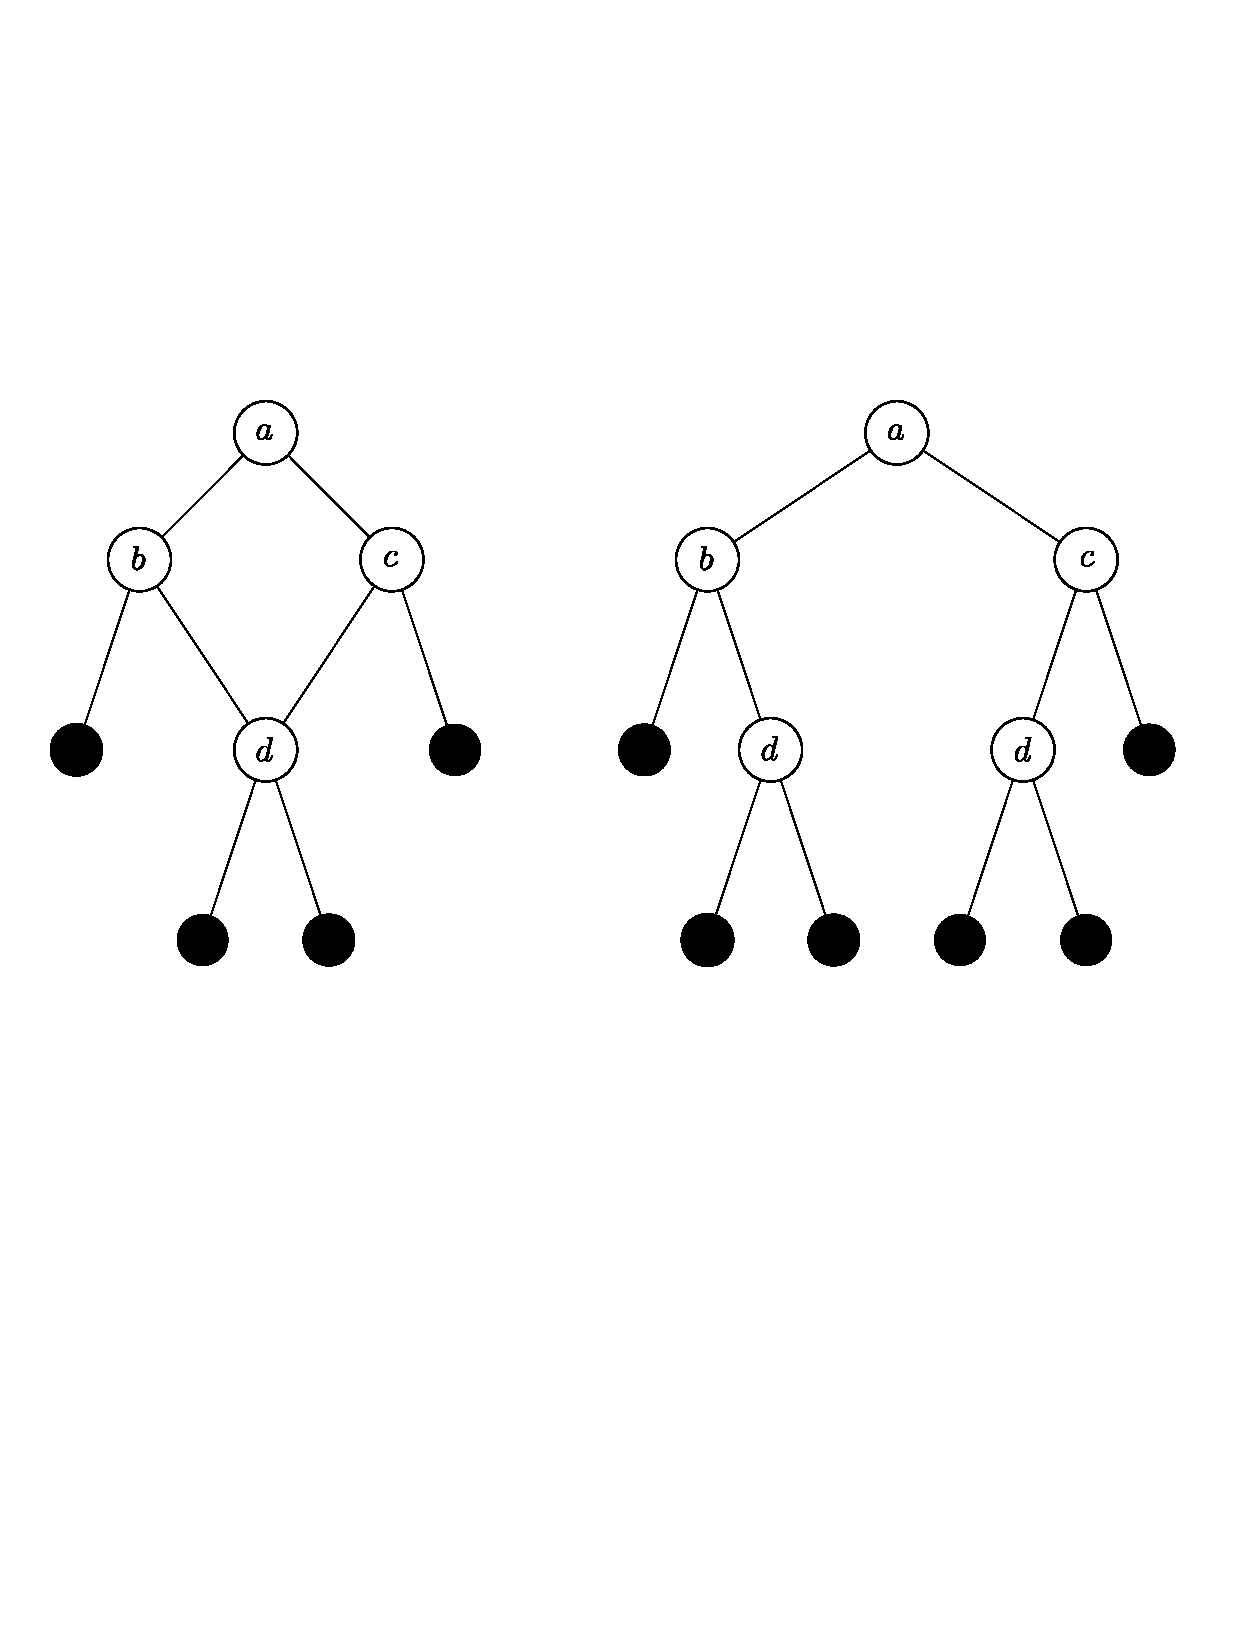
\includegraphics[trim = 0mm 10cm 0cm 0cm, clip, width=9cm]{treevsgraph.pdf}
\caption{Directed acyclic graph with corresponding tree.}
\label{treevsgraph}
\end{figure}

Above mentioned method solves the problem of repititions, but not transpositions. This second type of duplicate positions in the game tree
can still cause it to become very large. Figure \ref{treevsgraph} shows an example of a transposition. The so called \emph{join node} $d$ is
reachable via $b$ as well as $c$. The tree representation containing this transposition shows that $d$ and all its children occur multiple times.
If a node has join nodes amongst its ancestors in the DAG, it will
occur multiple times in the corresponding tree. The number of times it will occur in the tree can even depend exponentially on the amount of join
nodes.

Representing the search tree internally as a graph prevents this exponential behaviour. While this completely solves the issue of duplicate
positions, efficient draw detection becomes less trivial. Additionally, since proof-number search was designed for trees, this also means
the algorithm would have to be adapted.
Though it has been shown that proof-number search can still perform quite good on directed acyclic graphs without any adaptation,
on cyclic graphs it has to be adapted and can still give incorrect results ~\cite{Schijf93}.\\

\subsection{Implementations}
To test and compare the applicability of proof number search on small variants of shogi, taking into account the considerations on graphs and trees,
three algorithms were implemented. Most importantly are two variants of proof number search. These are proof number search with the search tree
represented as a tree and proof number-number search with the search tree represented as a graph.
To relativate the results of these two algorithms, a simple breadth first search is also implemented.

\paragraph{Proof-number search: tree.} This algorithm is exactly as explained in  as explained in Section \ref{pnsearch}. Draw is detected by running
the algorithm twice; in the first run black loses in drawing situations and in the second run white loses in those situations.

\paragraph{Proof-number search: graph.} In this variant the search tree is represented as a graph. The algorithm is the same except for the updating
procedure given in Algorithm \ref{alg:update}. In stead of only updating one parent, all parents have to be updated. Therefor, after expanding a
node $v$, all simple paths from $v$ to the root are updated. As trees are a special case of graphs, this is actually what also happens in the original
algorithm. Draw is detected if the complete search tree is expanded and the game has not been proved.

\paragraph{Breadth-first search.} As the name suggests, a simple breadth-first expansion of the search tree using the minimax method of determining
the game theoretical value of nodes. For this algorithm we also use a graph representation. Simalar to the proof-number search variant, it
updates all simple paths from the last expanded node $v$ to the root. It also detects draw by exhausting the search tree.

\section{Results}
\label{sec:results}
%Compare results of the three algorithms (BFS, PN on graph, PN on tree) and explain the differences.\\
%subsection: Point out where and why PN fails where BFS succeeds.
The first series of tests were performed on a $3 \times 3$ board with up to four pieces per player, always including exactly one king. To compensate
for the small board, both the rook and the bishop can only move one square in their usual directions and they can not promote. Each player
has four possible starting squares for their pieces as shown in Figure \ref{3x3setup}.
Eight different piece types led to an enumeration of 1372 different starting positions.
See Appendix \ref{3x3rules} for a detailed description of the rules for the $3 \times 3$-variants.

There are bound to be trivial games amongst the 1372 different starting positions. For instance, the king might be in check at the start, so since
the game is symmetrical the starting player will win. To filter out these situations we will only look at the games which needed an
average of 30 expanded nodes per algorithm to prove the value of the root. After filtering out the trivial games, 513 remain. Of these, 311 result
in a win for black, 180 in a win for white and 22 games which result in a draw. Table \ref{table:3x3result} shows some results from running the three
algorithms.

\begin{table}[h]
\begin{tabular}{| l | c | c | c | c |}
\cline{2-5}
 \multicolumn{1}{c|}{} & \multirow{2}{*}{Instances solved} & \multicolumn{3}{c|}{Average number of nodes expanded}\\
 \multicolumn{1}{c|}{} &    & \multicolumn{1}{c}{All instances} & \multicolumn{1}{c}{Solved by png} & \multicolumn{1}{c|}{Non drawing} \\ \hline
pnt & 513 & 5531 & 1312 & 5098\\
png & 359 & 2790 & 889 & 2533\\
bfs & 510 & 227336 & 62125 & 158340\\
\hline
\end{tabular}
\label{table:3x3result}
\caption{Test results of running proof-number search with tree (pnt) and graph (png) representation and breadth-first search (bfs) on 513 $3 \times 3$
instances.}
\end{table}

The results show that proof-number search on trees managed to solve every instance, while the graph variant solves considerably less. The
breadth-first method only failed to prove three instances, in all cases because of memory constraints ($\pm8$ million nodes) in trying to prove a draw.
Indeed, on average BFS expands several orders of magnitude more nodes than both PN variants. BFS used $\pm6.5$ million nodes to solve the hardest
game, whereas PN-search with tree representation only needed $\pm295\,000$. Looking only at games which did not result in draw (i.e. games where
BFS does not exhaustively searches the graph), BFS still consistently expands significantly more nodes than PN-search.

The difference in nodes expanded between PN-search on tree or on graphs is not so drastical
on this small scale; the graph variant uses about half of the tree variant (31029 vs. 58757 in the hardest game solved by using a graph).
The difference in solving capability however is more pronounced. Of the hundred hardest games, a mere third was proved by the graph variant.
One reason for this became evident when inspecting the most proving node after every cycle. The algorithm successively selected the same
node as most proving, which resulted in a loop.

\paragraph{Animal shogi.} The second series of test were performed on a commercial variant of shogi designed for children. It is played on a $3 \times 4$
board with a king, rook, bishop and pawn for each player.
The game is similar to the smaller $3 \times 3$ variant with the additional rule that reaching the promotion zone with your king wins you the game.
The full set of rules is explained in Appendix \ref{dobutsu}. This variant has been strongly solved
\cite{tetsuroanimal}, so it is a good test subject. The game has $\pm1.5$ billion reachable positions, which means that the game tree represented as a graph has exactly
this amount of nodes. It has been shown that white has a winning strategy. The longest game in which black
delays loss as long as possible and white tries to win as fast as possible has 78 plies; 39 moves per player. 

We will use the complete Animal shogi setup, as well as all variations where some pieces are missing (except the king). In all starting positions, black and white have the
same pieces missing. In Table \ref{animalresult} are the results of running PN-search with the tree representation on all the variations. The column with collisions shows that
in all but the simplest game a lot of positions are expanded more than once. In the game without pawn and bishop, the algorithm only expanded $19\,996$ unique positions
when it needed more than $4$ million to prove the root.

In the unproved games, the proof and disproof numbers were always strictly increasing in intervals of thousand iterations. In the $3 \times 3$ variants,
the algorithm would quickly proof the root once both proof and disproof numbers started to decline. \\

\begin{table}
\begin{tabular}{| l | c r@{.}l c c |}
\hline
 Missing & Nodes & \multicolumn{2}{c}{Collision \%} & PN & DN\\ \hline
 None                   & 11\,011\,553  & \quad~68&88 & 1\,298   & 1\,503\\
 Pawn                   & 12\,309\,114  & 92&63 & 1\,117   & 2\,017\\
 Bishop                 & 11\,176\,128  & 90&30 & 1\,003   & 1\,977\\
 Rook                   & 10\,939\,358  & 94&14 & 1\,200   & 1\,816\\
 Pawn \& Bishop         & 4\,130\,631   & 99&52 & $\infty$ & 0\\
 Bishop \& Rook         & 38\,879       & 71&09 & 0        & $\infty$\\
 Pawn \& Rook           & 28\,952       & 86&87 & $\infty$ & 0\\
 Pawn \& Bishop \& Rook & 63            & 0&0      & 0       & $\infty$\\
\hline
\end{tabular}
\caption{Test results of PN-search on Animal shogi.}
\label{animalresult}
\end{table}

Both algorithms using a graph representation only managed to prove the game with just two kings, which is a trivial 3-move win for black. BFS ran out of memory on all
but the one it solved. PN-search with a graph representation would quickly loop by selecting the same node as the most proving node.

\section{Discussion}
\label{sec:disc}

Even though PN-search was succesfully used to solve mating problems, even very large ones, the implementation as presented here did not show promising results. As the implementation
was not optimised for efficient memory usage, we did not expect to solve much more than small sized variants. However, the results from Animal shogi show that there are more -- maybe
more important -- ways than mere code optimisation to save memory.

%TODO fix this
One of the reasons PN-search fails on graphs is when the most proving node is not an unexpanded node. This happens when a node is part of a cycle
and the only node left to complete its proof is itself. If such a node is selected, it will be selected in the next round as well, resulting
in an infinite loop. As stated in Section \ref{sec:treegraph}, an adaptation of the PN-search algorithm has been proposed that (amongst others)
solves this problem. However even that improved version of PN-search on cyclic graphs disfunctions in certain situations.


\begin{itemize}
	\item Even very small instances of shogi are quite complex, give figures on number of nodes in proven drawn games.
	\item PN search not really fitted for non-destructive games
	\item Are there other viable methods for proving small games? How do they differ from PN search? Reduce nodes by domination simulation, then retrograde analysis.
\end{itemize}

{\appendix
\section{Shogi on a $3 \times 3$ board.}
\label{3x3rules}
\paragraph{Board size.} These shogi variants are played on a $3 \times 3$ board.

\paragraph{Setup.} Each player has up to four pieces always including a king. The starting positions for each player are shown in
Figure \ref{startingpos}.
\begin{figure}[h]
\center
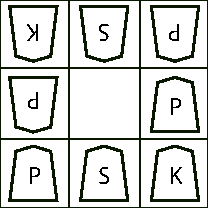
\includegraphics{smallsetup.pdf}
\caption{Black pieces point up, white pieces point down; in this example both players have one king (K), two pawns (P) and one silver general (S).}
\label{startingpos}
\end{figure}

\paragraph{Winning condition.} A player wins if the enemy king is captured. This usually means that both players try to checkmate the enemy's king, however an
inattentive player might accidentally make a move which leaves his king in check.

\paragraph{Promotion.}  A player's promotion zone is the furthest rank opposed to its pieces starting location. 
If a player moves a piece to, from or in the promotion zone he may chose to promote that piece if it can be promoted. If a piece has no more legal moves
(e.g. a pawn moving to the last rank) then it has to be promoted. A piece loses its current move set and gains the promoted move set upon promotion. A promoted piece can never
promote.

\paragraph{Drop rule.} If a player captures a piece of the enemy, he takes the captured piece in its hand. In one of its subsequent turns, in stead of moving one of his
pieces on the board, he might choose to place one of the pieces in his hand on the board. He can only place pieces on vacant squares. It is not allowed to place a piece
on the board such that it has no more legal moves, e.g. placing a pawn on the last rank is forbidden. If a piece is dropped in the promotion zone, it is \emph{not} promoted.
If that piece is moved in a subsequent turn however, normal promotion rules apply.

\paragraph{Pieces.} There are eight different pieces, each with a unique move set. Some pieces can promote while others can not. All pieces can capture enemy pieces with their normal movement
(unlike pawns in western chess).\\
\begin{tabular}{l l}
\textbf{King} & The same as in chess, one step in all directions.\\
\textbf{Bishop} & Normally the same as in chess, but here restricted to only one step diagonally.\\
\textbf{Rook} & Normally same as in chess, but here restricted to only one step orthogonally.\\
\textbf{Gold} General & One step in all directiones, except diagonally backwards.\\
\textbf{Silver} General & One step in all directions, except orthogonally backwards and sidewards.\\
\textbf{Knight} & Can move one step forwards plus one step diagonally forwards in one turn, possibly jumping over other pieces.\\
\textbf{Pawn} & One step forwards.\\
\end{tabular}
The Silver General, Knight and Pawn can promote. Their promoted move set is the same as the Gold General's.

\section{Animal shogi}
\label{dobutsu}

\paragraph{Board size.} This shogi variant is played on a $3 \times 4$ board.

\paragraph{Setup.} Each player has one king, bishop, rook and pawn. The starting setup is shown in Figure \ref{dobutsusetup}.
\begin{figure}[h]
\center
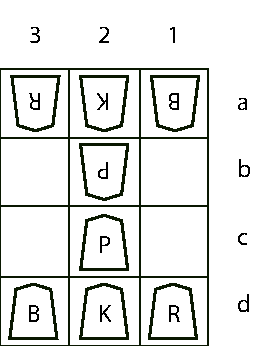
\includegraphics{dobutsushogi.pdf}
\caption{Starting setup for Animal shogi. Each player has a king (K), bishop (B), rook (R) and a pawn (P).}
\label{dobutsusetup}
\end{figure}

\paragraph{Winning condition.} A player wins if the enemy king is captured. Additionally, if a player moves his king to a square in the promotion zone
which is not under attack, that player wins. A square is under attack if the enemy can move one of its pieces there (excluding drops).

\paragraph{Promotion.}  A player's promotion zone is the furthest rank opposed to its pieces starting location. If a player moves a pawn to the promotion zone it will
always promote. Other pieces can not promote in this variant.

\paragraph{Drop rule.} If a player captures a piece of the enemy, he takes the captured piece in its hand. In one of its subsequent turns, in stead of moving one of his
pieces on the board, he might choose to place one of the pieces in his hand on the board. He can only place pieces on vacant squares. It is not allowed to place a pawn
in the promotion zone, as it will not promote and have no legal moves left.

\paragraph{Pieces.} There are four different pieces, each with a unique move set. Only the pawn can promote. All pieces can capture enemy pieces with their normal movement
(unlike pawns in western chess).\\
\begin{tabular}{l l}
\textbf{King} & The same as in chess, one step in all directions.\\
\textbf{Bishop} & One step diagonally.\\
\textbf{Rook} & One step orthogonally.\\
\textbf{Pawn} & One step forwards. Promotes to a Tokin.\\
\textbf{Tokin} & All directions except diagonally backwards.\\
\end{tabular}

}
\bibliography{cites}{}
\bibliographystyle{plain}

\end{document}
